%!TEX program = xelatex
% 使用 ctexart 文类,UTF-8 编码
\documentclass[UTF8]{ctexart}
\usepackage{cite}
\usepackage{geometry}
\usepackage{graphicx}
\usepackage[colorlinks,
            linkcolor=red,
            anchorcolor=blue,
            citecolor=green
            ]{hyperref}
\geometry{a4paper,scale=0.8}
\begin{document}
面试问题总结
\begin{abstract}
    在开发面试中,会遇到各种各样的问题,这里我们对面试中遇到的问题进行总结,方便自己经常性的反思和理解一些算法和常见的问题。帮助后续的程序面试的复习。
\end{abstract}
\section{魔鬼问题}
\subsection{题目}
现在有10个人被一个魔鬼逮住了。魔鬼对于直接把人杀掉的方法不感兴趣了。于是,他就想了一个杀人的新花样。
是这样的,一天晚上,魔鬼向这十个人宣布了游戏规则 ,即明早他要把他们10个人排成一排,然后从一堆既有无限多的
白帽子混会着无限多的黑帽子的帽子堆里为每个人随机抽取一顶帽子,给他们10个人都戴上帽子。因为 10个人是排成一
排的,所以排在第10个的人可以看到前面9个人帽子的颜色,排在第9个人可以看到前面8个人的帽子的颜色,...以此类推。然后,魔鬼会从排在 第10个人开始,问他,你头上的帽子的颜色是白色还是黑色,如果答对了,就放他走;如果答错了,
就被杀掉。然后同样问排在第9位的人,然后问同样问排在第8位的 人,...以此类推。在这其中,10个人所能做的只有当他
被魔鬼问到的时候,答白色或者黑色。不能有超越此范围的任何行动,不然,魔鬼会把他们10个人全都杀死 。 现在,魔鬼
给他们10个人一个晚上的时间去商量一个对策,使得他们中能存活下来的人越多越好。请问,你会有什么样的对策,请计
算出按照你的对策执行时最坏的情况 下,他们中能有多少人能100\%够活下来?期望能活下来的人数又是多少?
\subsection{思路}
 让答的人给前面的人足够多的信息
 \subsection{解答}
从只能回答白或黑,也就是只能2中选1,从而联想到二进制和奇偶性。二进制一下子没想出什么好方法,奇偶性有一些提
示,所以从奇偶性入手。第10个人 以他所见到的9个帽子中白帽的数量的奇偶性作答,例如大家约定白代表偶,黑代表奇,
则第10个人的回答是前9个帽子中白帽的数量的奇偶。他自己有50%的机会。 第9个人听到他的回答后,结合他看到的8顶帽
子中白帽的奇偶,可以知道自己的帽子的颜色,如实作答。第8个人知道9顶帽子中白帽的奇偶,加上听到第9顶帽子的颜 
色,就可以知道前8顶帽子中白帽的奇偶(如果第9个人答白,则前8顶中的白帽奇偶性与第第10个人所说的相反;如果第9
个人答黑,则相同),再结合所看到前7顶 帽子中的白帽数量,也可以推出自己的帽子颜色,也如实作答。依此类推
,前9个人都可以活下来,第10个人有一半机会。
\section{问题}
\subsection{问题}
给一个超过100G大小的log file, log中存着IP地址, 设计算法找到出现次数最多的IP地址?
与上题条件相同,如何找到top K的IP?如何直接用Linux系统命令实现?
\subsection{解答}
Hash分桶法: 
• 将100G文件分成1000份,将每个IP地址映射到相应文件中:$file_id = hash(ip) \% 1000 $
• 在每个文件中分别求出最高频的IP,再合并 Hash分桶法: 
• 使用Hash分桶法把数据分发到不同文件 
• 各个文件分别统计top K 
• 最后Top K汇总 
Linux命令,假设$top 10:sort log_file | uniq -c | sort -nr k1,1 | head -10$
\section{http和https的区别}
\subsection{Http和Https的基本概念}

Http:超文本传输协议(Http,HyperText Transfer Protocol)是互联网上应用最为广泛的一种网络协议。
设计Http最初的目的是为了提供一种发布和接收HTML页面的方法。它可以使浏览器更加高效。Http协议是以明文
方式发送信息的,如果黑客截取了Web浏览器和服务器之间的传输报文,就可以直接获得其中的信息。

Https:是以安全为目标的Http通道,是Http的安全版。Https的安全基础是SSL。SSL协议位于TCP/IP协议与各
种应用层协议之间,为数据通讯提供安全支持。SSL协议可分为两层:SSL记录协议(SSL Record Protocol),它
建立在可靠的传输协议(如TCP)之上,为高层协议提供数据封装、压缩、加密等基本功能的支持。SSL握手协议(SSL 
Handshake Protocol),它建立在SSL记录协议之上,用于在实际的数据传输开始前,通讯双方进行身份认证、协商
加密算法、交换加密密钥等。
\subsection{Http与Https的区别}
1、https协议需要到CA申请证书,一般免费证书较少,因而需要一定费用。(原来网易官网是http,而网易邮箱
	是https。)

2、http是超文本传输协议,信息是明文传输,https则是具有安全性的ssl加密传输协议。

3、http和https使用的是完全不同的连接方式,用的端口也不一样,前者是80,后者是443。

4、http的连接很简单,是无状态的。Https协议是由SSL+Http协议构建的可进行加密传输、身份认证的网络协议,
比http协议安全。(无状态的意思是其数据包的发送、传输和接收都是相互独立的。无连接的意思是指通信双方都不
	长久的维持对方的任何信息。)
\subsection{Https的优点}
1、使用Https协议可认证用户和服务器,确保数据发送到正确的客户机和服务器。

2、Https协议是由SSL+Http协议构建的可进行加密传输、身份认证的网络协议,要比http协议安全,可防止数据在
传输过程中不被窃取、修改,确保数据的完整性。

3、Https是现行架构下最安全的解决方案,虽然不是绝对安全,但它大幅增加了中间人攻击的成本。
\subsection{Https的缺点(对比优点)}
1、Https协议握手阶段比较费时,会使页面的加载时间延长近。

2、Https连接缓存不如Http高效,会增加数据开销,甚至已有的安全措施也会因此而受到影响;

3、SSL证书通常需要绑定IP,不能在同一IP上绑定多个域名,IPv4资源不可能支撑这个消耗。

4、Https协议的加密范围也比较有限。最关键的,SSL证书的信用链体系并不安全,特别是在某些国家可以控制CA根
证书的情况下,中间人攻击一样可行。
\subsection{Https的连接过程}
\begin{figure}[htbp]
\centering
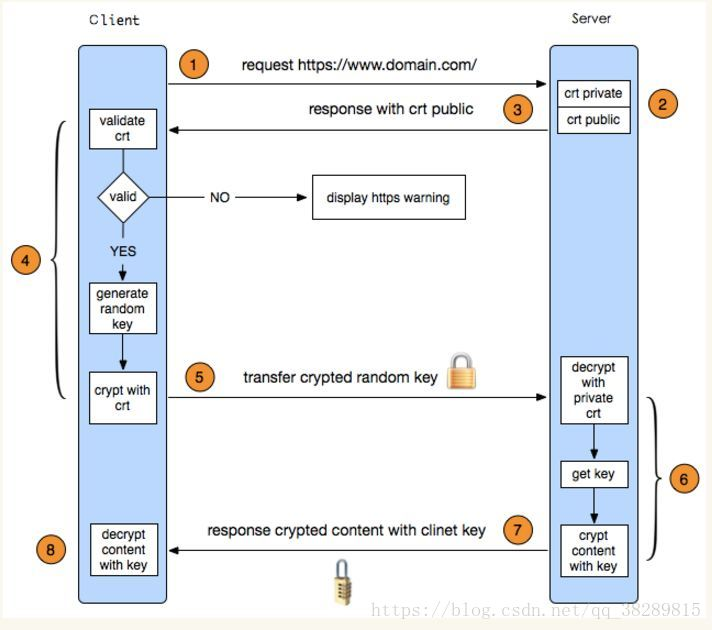
\includegraphics[height=6.0cm,width=9.5cm]{Figure/20180709141944471.jpg}
\caption{Https的连接过程}
\end{figure}
图片中的过程是按8个步骤分的,但是网上有更详细的步骤,所以我把详细的过程和这个图片配在一起。

①客户端的浏览器向服务器发送请求,并传送客户端SSL 协议的版本号,加密算法的种类,产生的随机数,以及其他
服务器和客户端之间通讯所需要的各种信息。

②服务器向客户端传送SSL 协议的版本号,加密算法的种类,随机数以及其他相关信息,同时服务器还将向客户端传
送自己的证书。

③客户端利用服务器传过来的信息验证服务器的合法性,服务器的合法性包括:证书是否过期,发行服务器证书的CA
 是否可靠,发行者证书的公钥能否正确解开服务器证书的“发行者的数字签名”,服务器证书上的域名是否和服务器
 的实际域名相匹配。如果合法性验证没有通过,通讯将断开;如果合法性验证通过,将继续进行第四步。

④用户端随机产生一个用于通讯的“对称密码”,然后用服务器的公钥(服务器的公钥从步骤②中的服务器的证书中获得)
对其加密,然后将加密后的“预主密码”传给服务器。

⑤如果服务器要求客户的身份认证(在握手过程中为可选),用户可以建立一个随机数然后对其进行数据签名,将这个
含有签名的随机数和客户自己的证书以及加密过的“预主密码”一起传给服务器。

⑥如果服务器要求客户的身份认证,服务器必须检验客户证书和签名随机数的合法性,具体的合法性验证过程包括:客
户的证书使用日期是否有效,为客户提供证书的CA 是否可靠,发行CA 的公钥能否正确解开客户证书的发行CA 的数字
签名,检查客户的证书是否在证书废止列表(CRL)中。检验如果没有通过,通讯立刻中断;如果验证通过,服务器将用
自己的私钥解开加密的“预主密码”,然后执行一系列步骤来产生主通讯密码(客户端也将通过同样的方法产生相同的主
通讯密码)。

⑦服务器和客户端用相同的主密码即“通话密码”,一个对称密钥用于SSL 协议的安全数据通讯的加解密通讯。同时在SSL
通讯过程中还要完成数据通讯的完整性,防止数据通讯中的任何变化。

⑧客户端向服务器端发出信息,指明后面的数据通讯将使用的步骤⑦中的主密码为对称密钥,同时通知服务器客户端的握
手过程结束。

⑨服务器向客户端发出信息,指明后面的数据通讯将使用的步骤⑦中的主密码为对称密钥,同时通知客户端服务器端的握
手过程结束。

⑩SSL 的握手部分结束,SSL 安全通道的数据通讯开始,客户和服务器开始使用相同的对称密钥进行数据通讯,同时进行
通讯完整性的检验。


\section{Data Acquisition}

\section{南京大学计算机学院}

\subsection{Apple}
南京大学计算机科学与技术系,是国家级重点的计算机系,在人工智能研究和形式化方法研究上居于世界领先地位,是国内首屈一指的计算机系。
\subsection{模型驱动建模}
模型驱动建模是一个关键的软件建模技术,在软件开发领域占有重要的应用。模型$G=(U,V)$
\bibliographystyle{plain}
\bibliography{ref}
\end{document}